	\clearpage
\section{Konzept}\label{sec:Konzept}

Für den Vergleich der 3 Mesh Netzwerkstack Bluetooth Mesh (BT Mesh), Thread und Zigbee soll folgendes vom Protokoll unabhängiges Testkonzept umgesetzt werden. 
Die Abbildung \ref{fig:MeshTestkonzept} zeigt das Konzeptschema. Die Benchmark Slave Nodes (BSN) in der Abbildung als Sensoren und Aktoren mit unterschiedlichen Funktionalitäten dargestellt, bilden zusammen mit dem Benchmark Master Node (BMN) das zu testende Mesh Netzwerk. Innerhalb des Netzwerks wird dessen Organisation vom jeweiligen Protokoll sichergestellt. 
Die Benchmark Management Station (BMS) welche mit dem BMN via USB/UART kommuniziert ist zuständig für die Verwaltung und Verarbeitung der Benchmarks. Während eines Benchmark Prozesses sollen sämtliche Messungen jedoch unabhängig von der BMS durchgeführt werden damit allfällige Latenzzeiten der USB/UART Verbindung die Resultate nicht verfälschen.
Das Mesh Testnetzwerk soll unter unterschiedlichen Bedingungen betrieben. Diese Testszenarien werden unter \ref{sec:Testszenarien} genauer beschrieben.



%\begin{itemize}
% 	\item Punkt-Punkt Testinfrastrukturen auf MAC-Ebene
% 	\item Test Mesh Netzwerke für BT Mesh, Zigbee und Thread
% 	\item Steuer- und Auswertesoftware
%\end{itemize}



%\begin{figure}[H]
%	\centering
%	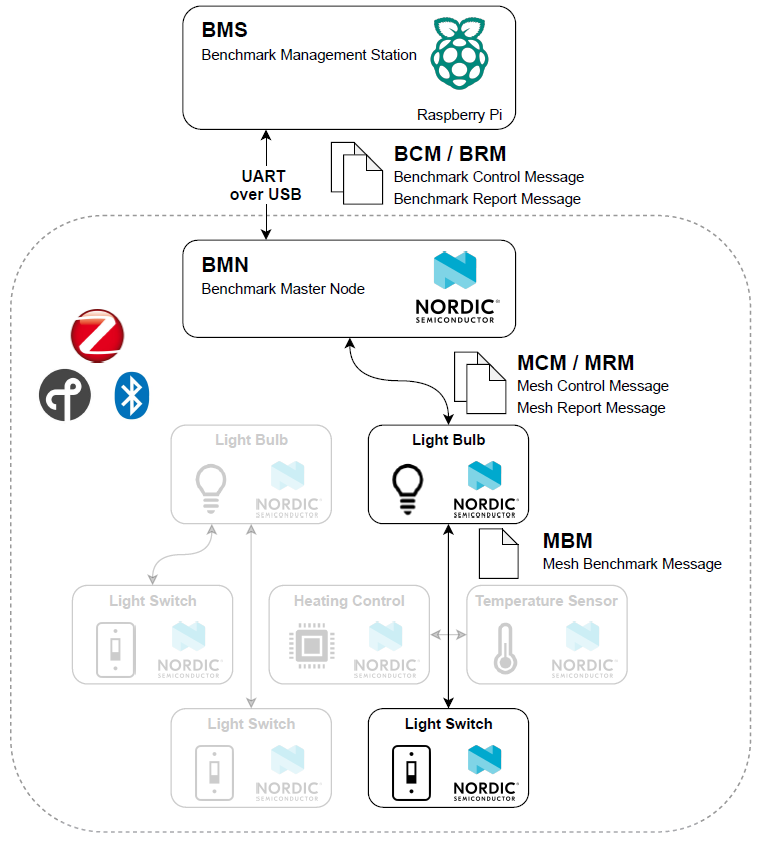
\includegraphics[width=1.0\textwidth]{Mesh_Testkonzept.png}
%	\caption{Konzeptschema Mesh Test Netzwerk}\label{fig:MeshTestkonzept}
%\end{figure}







